
\documentclass[
	8pt,
]{beamer}

\graphicspath{{Images/}{./}} 
\usepackage{booktabs} 
\usetheme{Madrid}

\usefonttheme{structurebold} 
\useinnertheme{rounded}

\title[OfflineDataSci]{Overview: Offlinedatasci automates the downloading and updating of the most recent materials for running workshops.}

\subtitle{Optional Subtitle} 

\author[VC EPW JSS CS AD]{VC EPW JSS CS AD} 

\date[\today]{\today}
\begin{document}

\begin{frame}
	\frametitle{OfflineDataSci} % Slide title, remove this command for no title
	\framesubtitle{A Python Package for Managing Common Data Science Tools for Carpentries Workshops or Individual Users When Limited Access to the Internet is Anticipated}
	\begin{block}{Introduction}
	Overview: Offlinedatasci automates the downloading and updating of the most recent materials for running workshops.
	\end{block}	
	\begin{columns}[t]
		\begin{column}{0.6\textwidth} % Left column width
		
			\begin{itemize}
   				\item Limited internet access is an obstacle for data science workshop attendees, individual learners, and practitioners.
       
				\item OfflineDataSci is a Python package with a command-line interface that allows workshop instructors or individuals to maintain local teaching servers or local work environments.
				
				\item It downloads lesson materials for Software, Data, and Library Carpentries; installers for essential tools like \textbf{R}, \textbf{Python}, and \textbf{Rstudio}; and creates local mirrors of the R and Python package repositories that can be customized.
    
			\end{itemize}
		\end{column}
		
		\begin{column}{0.4\textwidth} % Right column width
			\begin{figure}
				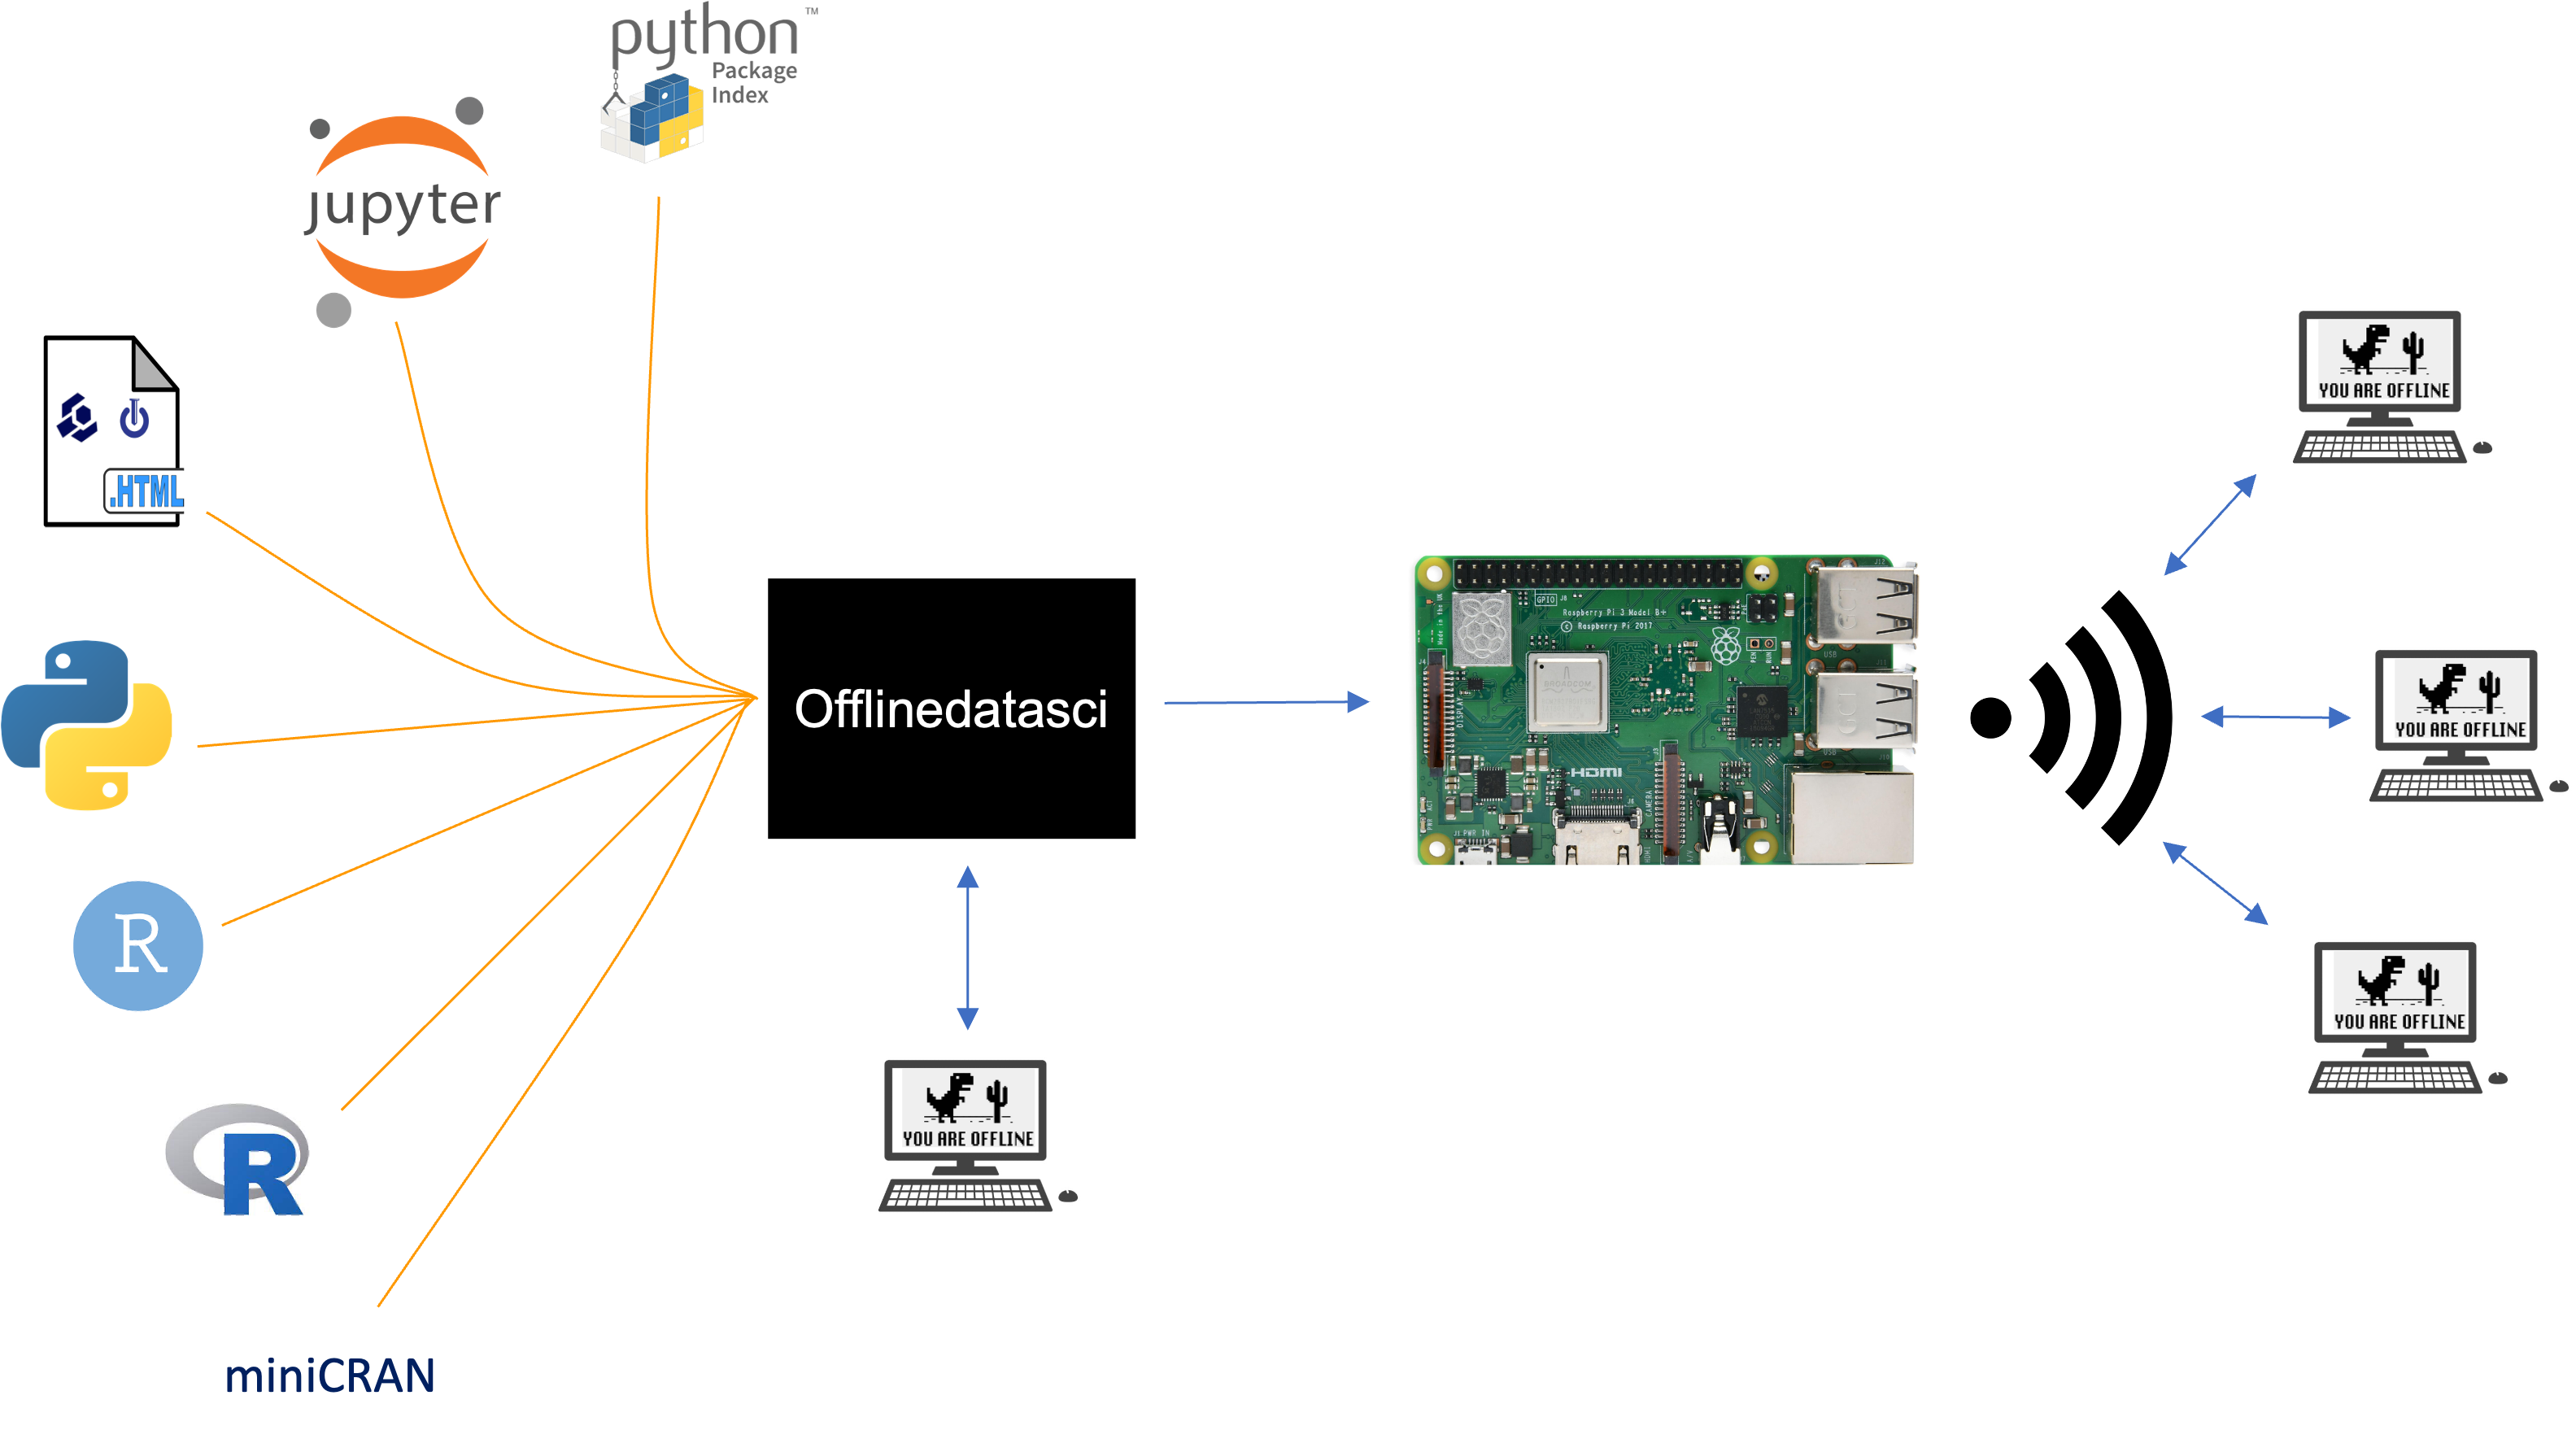
\includegraphics[width=1\linewidth]{offlinedatasci.png}
				\caption{OfflineDataSci handles downloading and configuring software and lessons.}
			\end{figure}
		\end{column}
	\end{columns}
	\begin{block}{Acknowledgements}
		Virnaliz Cruz, Ethan P. White, Jannetta S. Steyn, Colin Sauze, Abhishek Dasgupta
	\end{block}
\end{frame}


\end{document} 
